\documentclass{article}

\usepackage{fontspec}
\usepackage{fullpage}
\usepackage{multicol}
\usepackage{multirow}
\usepackage{tikz}

\begin{document}

\newfontfamily\swfill{SuttonSignWritingFill.ttf}
\newfontfamily\swline{SuttonSignWritingLine.ttf}
\newcommand{\bul}{\hfil$\bullet$&}
\renewenvironment{glossary}{\begin{multicols}{5}\begin{center}}{\end{center}\end{multicols}}
\setcounter{secnumdepth}{0}
\setlength{\columnseprule}{1pt}

\section{Supplement For Lesson 4}

\begin{center}
\it
Objectives inspired by, vocabulary transcribed from, and sentences and story by Bill Vicars.

Handshape photos by Adam Frost.

No endorsement implied nor given by either.
\end{center}

\subsection{Objectives}

\begin{tabular}{p{1cm}p{14cm}}
\bul I have completed the objectives for this lesson.\\
\bul I know how SignWriting handles non-manual markers.\\
\bul I am able to demonstrate the iconicity of SignWriting.\\
\bul I understand how directionality affects SignWriting.\\
\bul I am able to read the numbers 21--30.\\
\bul I am able to show the meaning and form of the symbol group in the timing category.\\
\bul I understand which types of handshapes are in Symbol Groups six and seven.\\
\bul I am able to draw the side palmshape in all forms.\\
\bul I am able to draw and demonstrate what fill three means.\\
\bul I am able to read, write, and sign half of the ASL handshapes in symbol group three.\\
\bul I am able to recognize the vocabulary for this lesson.\\
\bul I am able to read the practice sentences for this lesson.\\
\bul I am able to read the practice story for this lesson.\\
\end{tabular}

\subsection{Non-Manual Markers}

You should think I'm being silly with bothering to mention this by now but here goes.

A non-manual marker is anything not (non-) on the hands (manual), which we have seen quite a bit already.
Things like the B518x518S30a00482x483 meaning a yes or no question verses B518x518S30c00482x483 meaning a question to answer.

\subsection{The Iconicity of SignWriting}

When selecting a symbol for index finger extended, you could use a symbol like \tikz{\draw(0,0)circle(5pt);\filldraw(0,0)circle(1pt);} and just learn that it means index finger extended.
Given enough arbitrary symbols, this could be just as effective in recording ASL even if it took a little more memory at first.
There is nothing wrong with choosing to do this.

Instead, most of SignWriting has been designed to remind the reader and writer of what the item is.
All of the handshapes, movement, and faces have been designed to look like the actual hands, movement, and faces involved.

The handshapes even move where the fingers are drawn to match.
When you see B508x515S10000493x485 and B508x515S10010493x485, they both look very like your hand: in one case with the closed fingers to the left of your index and in the other with the fist to the left of your index.
Which is why the finger moves on B508x515S10020493x485, it now looks like where your actual finger is.

When looking at movement, knowing that B507x508S22a00494x493 is up while B507x508S26500493x493 is forward is an arbitrary remembering of stems, both B507x508S22a02494x493 and B507x508S26502493x493 are to the left and look like it.

And as for faces, you don't even really need to be told that B518x518S30a00482x483 means eyebrows up, it just looks like it.

This has the additional side-effect that ASL words which are iconic are also iconic in SignWriting.
B525x539S15a11502x476S15a19476x476S20500495x462S23904505x501S2391c477x501S2fb04494x533 looks like it might mean house, B531x538S14c10487x463S15a56470x526S37900497x492S2e208511x478 looks like a tree, and B535x539S14c00507x476S23108507x512S14c08470x488S23118468x522S22520503x461S22520465x474 looks like you are showing a fire.

\subsection{Directionality in SignWriting}

Most languages do something called conjugate --- that is change their form depending on either who is performing the action (the actor), or who the action is being perform on (the patient), or both.

English is of the first type --- I \emph{speak} to myself, she \emph{speaks} to me, I \emph{speak} to her, and she \emph{speaks} to herself.
If you know who the actor is then you can conjugate correctly regardless of the patient.

ASL is of that third type, that conjugates based on both.

\begin{center}
\begin{tabular}{*{4}{c}}
B514x552S10008486x480S10020492x487S20500504x485S26614487x449S26600491x522&B514x534S10008486x497S10020492x504S20500504x502S26614487x466&B514x536S10008486x464S10020492x471S20500504x469S26600491x506&B553x519S10008490x482S10020496x489S20500508x487S26616448x500S26602523x501\\
Meet&You meet me&I meet you&They meet\\
\end{tabular}
\end{center}

\subsection{The Numbers 21 through 30}

\begin{center}
\begin{tabular}{*{5}{c}}
\textbf{21}&\textbf{22}&\textbf{23}&\textbf{24}&\textbf{25}\\
B522x515S1e020499x485S21800479x503&
B518x524S10e50482x476S2890a489x509&
B519x517S12420481x487S22114493x484&
B525x516S1dc20476x486S14420503x485&
B521x514S1c510491x486S22124480x504\\
\textbf{26}&\textbf{27}&\textbf{28}&\textbf{29}&\textbf{30}\\
B523x516S1dc10477x485S18720505x487&
B525x516S1dc10476x485S1a520504x488&
B525x516S1dc10476x485S1bb20504x488&
B525x516S1dc10476x485S1ce20503x486&
B522x516S11e20478x485S17620506x500\\
\end{tabular}
\end{center}

\subsection{The Timing Category}

We informally call this category timing though it's official name is ``Dynamics \& Timing'' and has one base symbol in it.
The symbol groups can be thought of as three groups of ten, and here is where knowing the categories in order starts to help.

\begin{center}
\begin{tabular}{ccc}
\textbf{Symbol}\\
\textbf{Group}&\textbf{Name}&\textbf{Example}\\
\textbf{21}&Timing&B506x504S2f700494x497\\
\end{tabular}
\end{center}

With there only being one, and it having the same informal name (and official name) you should be able to remember it fairly easy but you technically don't have to yet.

\subsection{Symbol Groups Six and Seven}

The sixth Symbol Group we informally call six, though it's official name is ``Baby Finger''.
Symbol Group Baby Finger (Six) have all the handshapes where either the baby finger is extended or all fingers except the baby finger are extended.

The seventh Symbol Group we informally call seven, though it's official name is ``Ring Finger''.
Symbol Group Ring Finger (Seven) have all the handshapes where either the ring finger is extended or all fingers except the ring finger are extended.

Before you can consider this lesson complete, you need to be able to list off the symbol groups as:
``one, two, three, four, five, six, seven''

\subsection{The Side Palmshape}

\begin{center}
\begin{tabular}{r*{6}{c}}
&\textbf{Fill 1}&\textbf{Fill 2}&\textbf{Fill 3}&\textbf{Fill 4}&\textbf{Fill 5}&\textbf{Fill 6}\\
\textbf{Right}&
B512x508S18200489x493&
B512x508S18210489x493&
B512x508S18220489x493&
B512x508S18230489x493&
B512x508S18240489x493&
B512x508S18250489x493\\
\textbf{Left}&
B512x508S18208489x493&
B512x508S18218489x493&
B512x508S18228489x493&
B512x508S18238489x493&
B512x508S18248489x493&
B512x508S18258489x493\\
\end{tabular}
\end{center}

\subsection{The Third Fill}

\subsubsection{Hand Symbols}

\begin{center}
B508x515S10020493x485 B508x515S10e20493x485 B512x515S11e20489x485
\end{center}

Any symbol drawn in the third fill means that the signer's palm is facing away from the signer.
For all the hand symbols, the empty portion represents the signer's palm and the filled portion represents the back of the hand.
So for fill three, even if the hand was open you would only see the back of your hand --- leaving fill three completely filled symbol.

\subsubsection{Movement Symbols}

\begin{center}
B508x515S22b20492x485 B508x515S25620492x485 B508x515S26620492x485
\end{center}

Any symbol drawn in the third fill means that the both hands are doing the movement together, so these are all both hands moving.

\subsubsection{Everything Else}

\begin{center}
B506x504S2f720494x497 B518x518S30a20482x483 B537x504S38720463x496
\end{center}

The fills for other categories tend to be a bit more variable.
Here we have double-fast, left eyebrow raised, and slow comma.

\subsection{First ASL Handshapes From Symbol Group Three}

The twelve handshapes in Symbol Group Three used by ASL in order are:
{\it
Index Middle Thumb;
Index Middle Bent, Thumb Straight;
Index Middle Thumb Bent;
Index Up, Middle Hinge, Thumb Side;
Index Middle Thumb Cup;
}
Index Middle Thumb Circle;
Index Middle Unit, Thumb Side;
Index Middle Unit Hinge, Thumb Side;
Index Middle Cross, Thumb Side;
Middle Thumb Circle, Index Up;
Index Middle Thumb, Angle;
and Middle Thumb Angle Out, Index Up.

In case you hadn't noticed before, the \emph{italic} handshapes are the ones we are covering in this lesson.

\subsubsection{The Index Middle Thumb Handshape}

\begin{center}
\begin{tabular}{r*{6}{c}}
&\textbf{Fill 1}&\textbf{Fill 2}&\textbf{Fill 3}&\textbf{Fill 4}&\textbf{Fill 5}&\textbf{Fill 6}\\
\multirow{2}{*}{\textbf{Right}}&
B512x511S11e00488x489&
B512x511S11e10488x489&
B512x511S11e20488x489&
B512x511S11e30488x489&
B512x511S11e40488x489&
B512x511S11e50488x489\\
&
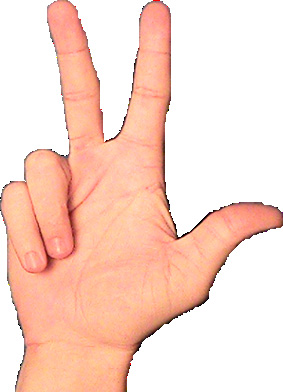
\includegraphics[scale=0.1]{images/03-01-1.jpg}&
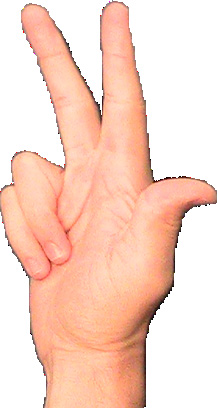
\includegraphics[scale=0.1]{images/03-01-2.jpg}&
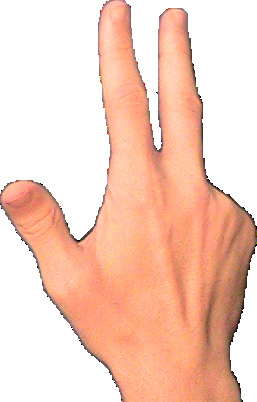
\includegraphics[scale=0.1]{images/03-01-3.jpg}&
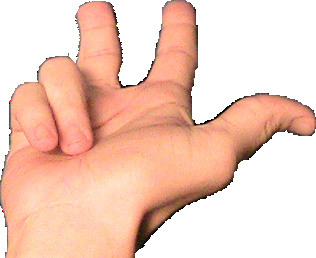
\includegraphics[scale=0.1]{images/03-01-4.jpg}&
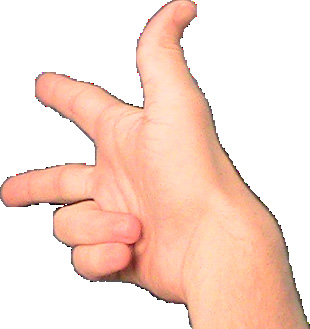
\includegraphics[scale=0.1]{images/03-01-5.jpg}&
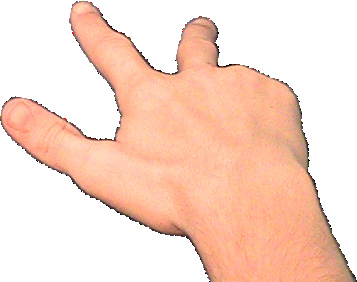
\includegraphics[scale=0.1]{images/03-01-6.jpg}\\
\textbf{Left}&
B512x511S11e08488x489&
B512x511S11e18488x489&
B512x511S11e28488x489&
B512x511S11e38488x489&
B512x511S11e48488x489&
B512x511S11e58488x489\\
\end{tabular}
\end{center}

\subsubsection{The Index Middle Bent, Thumb Straight Handshape}

\begin{center}
\begin{tabular}{r*{6}{c}}
&\textbf{Fill 1}&\textbf{Fill 2}&\textbf{Fill 3}&\textbf{Fill 4}&\textbf{Fill 5}&\textbf{Fill 6}\\
\multirow{2}{*}{\textbf{Right}}&
B512x511S12100488x489&
B512x511S12110488x489&
B512x511S12120488x489&
B512x511S12130488x489&
B512x511S12140488x489&
B512x511S12150488x489\\
&
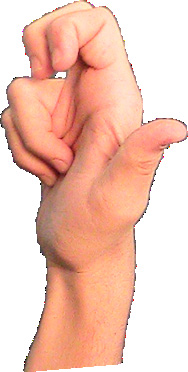
\includegraphics[scale=0.1]{images/03-02-1.jpg}&
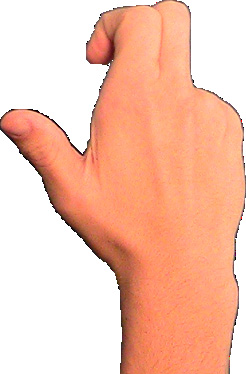
\includegraphics[scale=0.1]{images/03-02-2.jpg}&
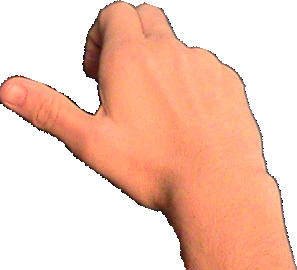
\includegraphics[scale=0.1]{images/03-02-3.jpg}&
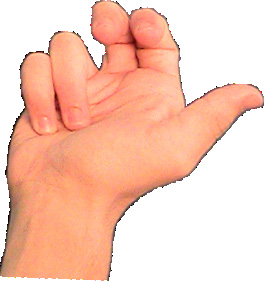
\includegraphics[scale=0.1]{images/03-02-4.jpg}&
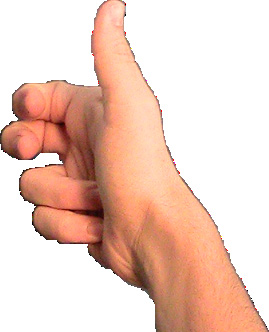
\includegraphics[scale=0.1]{images/03-02-5.jpg}&
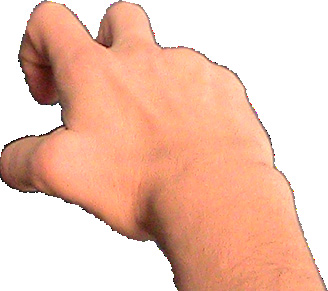
\includegraphics[scale=0.1]{images/03-02-6.jpg}\\
\textbf{Left}&
B512x511S12108488x489&
B512x511S12118488x489&
B512x511S12128488x489&
B512x511S12138488x489&
B512x511S12148488x489&
B512x511S12158488x489\\
\end{tabular}
\end{center}

\subsubsection{The Index Middle Thumb Bent Handshape}

\begin{center}
\begin{tabular}{r*{6}{c}}
&\textbf{Fill 1}&\textbf{Fill 2}&\textbf{Fill 3}&\textbf{Fill 4}&\textbf{Fill 5}&\textbf{Fill 6}\\
\multirow{2}{*}{\textbf{Right}}&
B512x511S12200488x489&
B512x511S12210488x489&
B512x511S12220488x489&
B512x511S12230488x489&
B512x511S12240488x489&
B512x511S12250488x489\\
&
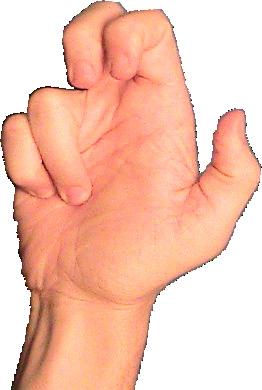
\includegraphics[scale=0.1]{images/03-03-1.jpg}&
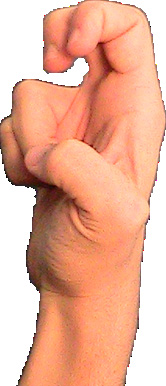
\includegraphics[scale=0.1]{images/03-03-2.jpg}&
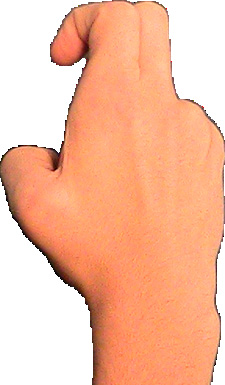
\includegraphics[scale=0.1]{images/03-03-3.jpg}&
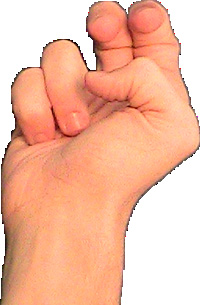
\includegraphics[scale=0.1]{images/03-03-4.jpg}&
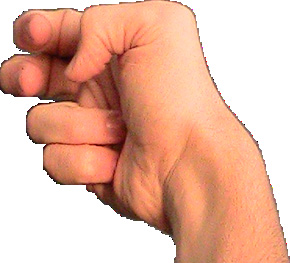
\includegraphics[scale=0.1]{images/03-03-5.jpg}&
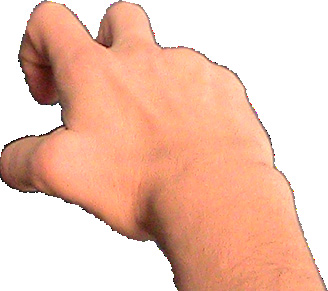
\includegraphics[scale=0.1]{images/03-03-6.jpg}\\
\textbf{Left}&
B512x511S12208488x489&
B512x511S12218488x489&
B512x511S12228488x489&
B512x511S12238488x489&
B512x511S12248488x489&
B512x511S12258488x489\\
\end{tabular}
\end{center}

\subsubsection{The Index Up, Middle Hinge, Thumb Side Handshape}

This symbol introduces a new concept in fills 1, 3, 4, and 6.

\begin{center}
\begin{tabular}{r*{6}{c}}
&\textbf{Fill 1}&\textbf{Fill 2}&\textbf{Fill 3}&\textbf{Fill 4}&\textbf{Fill 5}&\textbf{Fill 6}\\
\multirow{2}{*}{\textbf{Right}}&
B512x511S12400488x489&
B512x511S12410488x489&
B512x511S12420488x489&
B512x511S12430488x489&
B512x511S12440488x489&
B512x511S12450488x489\\
&
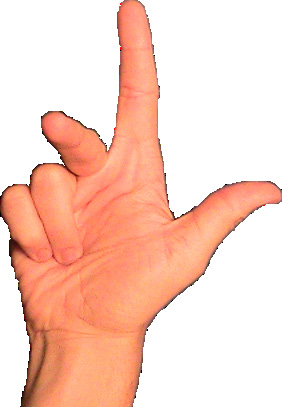
\includegraphics[scale=0.1]{images/03-04-1.jpg}&
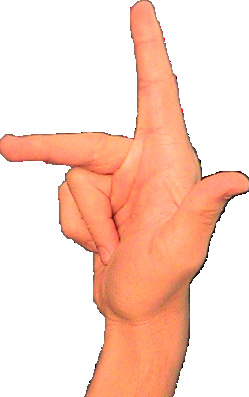
\includegraphics[scale=0.1]{images/03-04-2.jpg}&
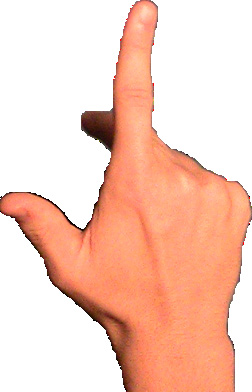
\includegraphics[scale=0.1]{images/03-04-3.jpg}&
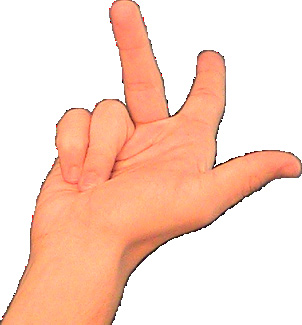
\includegraphics[scale=0.1]{images/03-04-4.jpg}&
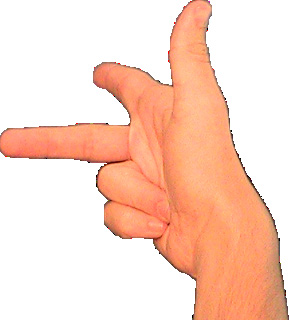
\includegraphics[scale=0.1]{images/03-04-5.jpg}&
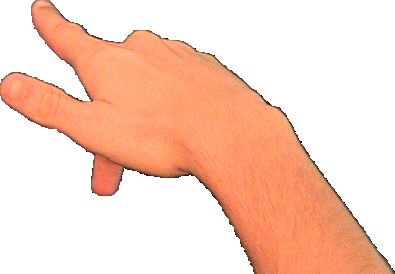
\includegraphics[scale=0.1]{images/03-04-6.jpg}\\
\textbf{Left}&
B512x511S12408488x489&
B512x511S12418488x489&
B512x511S12428488x489&
B512x511S12438488x489&
B512x511S12448488x489&
B512x511S12458488x489\\
\end{tabular}
\end{center}

When a finger (or thumb) is pointing at the signer in fill 1, the finger (or thumb) becomes a circle.
This convention matches with the diagonal movement that you will learn about later --- the circle means it is heading your direction.

Normally, something heading away from you would be a line, but for handshapes we don't do that for fills 3 and 6.
Instead we still use the circle to both match fills 1 and 4 and so that we won't confuse fill 3 with fill 6 or have to make sure our lines in fill 6 are separated ``enough'' to show.

%%%%%
When writing you are free to use either the circle or to use something that looks more like fills 2 and 5 --- whichever is easier for you, just like you can use ``g'' or {\em ``g''} in your writing of English.
Both are the same letter regardless of what you may see in print.

\subsubsection{The Index Middle Thumb Cup Handshape}

\begin{center}
\begin{tabular}{r*{6}{c}}
&\textbf{Fill 1}&\textbf{Fill 2}&\textbf{Fill 3}&\textbf{Fill 4}&\textbf{Fill 5}&\textbf{Fill 6}\\
\multirow{2}{*}{\textbf{Right}}&
B512x511S12800488x489&
B512x511S12810488x489&
B512x511S12820488x489&
B512x511S12830488x489&
B512x511S12840488x489&
B512x511S12850488x489\\
&
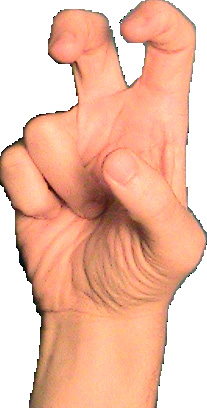
\includegraphics[scale=0.1]{images/03-05-1.jpg}&
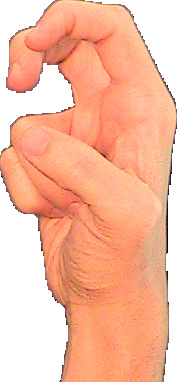
\includegraphics[scale=0.1]{images/03-05-2.jpg}&
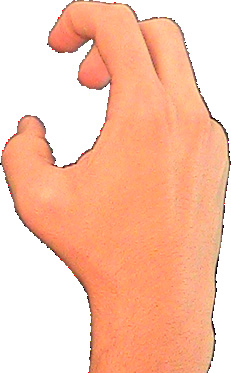
\includegraphics[scale=0.1]{images/03-05-3.jpg}&
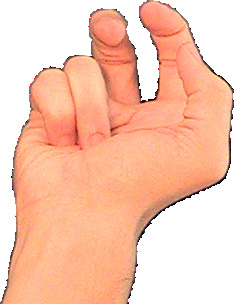
\includegraphics[scale=0.1]{images/03-05-4.jpg}&
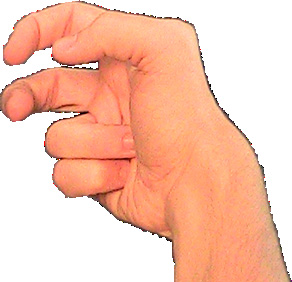
\includegraphics[scale=0.1]{images/03-05-5.jpg}&
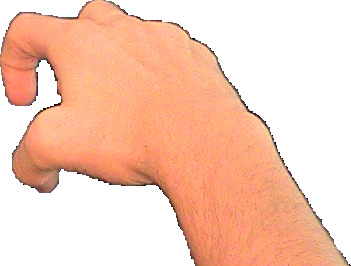
\includegraphics[scale=0.1]{images/03-05-6.jpg}\\
\textbf{Left}&
B512x511S12808488x489&
B512x511S12818488x489&
B512x511S12828488x489&
B512x511S12838488x489&
B512x511S12848488x489&
B512x511S12858488x489\\
\end{tabular}
\end{center}

\subsubsection{The Index Middle Thumb Circle Handshape}

\begin{center}
\begin{tabular}{r*{6}{c}}
&\textbf{Fill 1}&\textbf{Fill 2}&\textbf{Fill 3}&\textbf{Fill 4}&\textbf{Fill 5}&\textbf{Fill 6}\\
\multirow{2}{*}{\textbf{Right}}&
B512x511S12900488x489&
B512x511S12910488x489&
B512x511S12920488x489&
B512x511S12930488x489&
B512x511S12940488x489&
B512x511S12950488x489\\
&
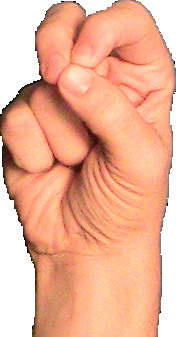
\includegraphics[scale=0.1]{images/03-06-1.jpg}&
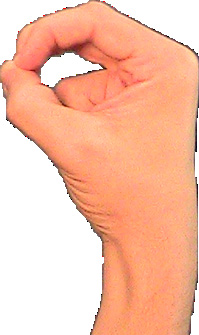
\includegraphics[scale=0.1]{images/03-06-2.jpg}&
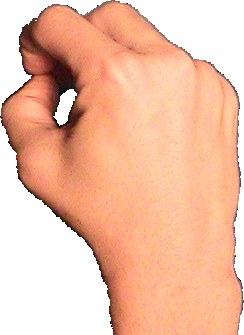
\includegraphics[scale=0.1]{images/03-06-3.jpg}&
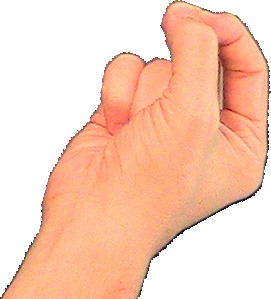
\includegraphics[scale=0.1]{images/03-06-4.jpg}&
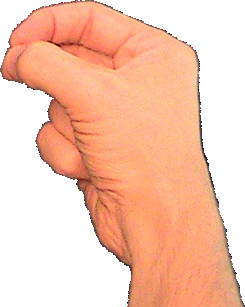
\includegraphics[scale=0.1]{images/03-06-5.jpg}&
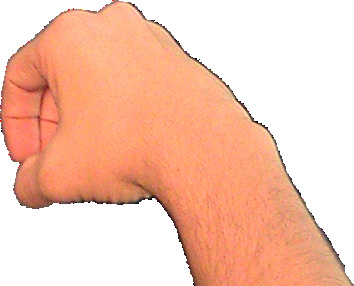
\includegraphics[scale=0.1]{images/03-06-6.jpg}\\
\textbf{Left}&
B512x511S12908488x489&
B512x511S12918488x489&
B512x511S12928488x489&
B512x511S12938488x489&
B512x511S12948488x489&
B512x511S12958488x489\\
\end{tabular}
\end{center}

\subsection{Vocabulary}

\begin{glossary}

\textbf{21}\\
AS1e020S21800M522x515S1e020499x485S21800479x503

\textbf{22}\\
AS10e50S2890aM518x524S10e50482x476S2890a489x509

\textbf{23}\\
AS12420S22114M519x517S12420481x487S22114493x484

\textbf{24}\\
AS1dc20S14420M525x516S1dc20476x486S14420503x485

\textbf{25}\\
AS1c510S22124M521x514S1c510491x486S22124480x504

\textbf{26}\\
AS1dc10S18720M523x516S1dc10477x485S18720505x487

\textbf{27}\\
AS1dc10S1a520M525x516S1dc10476x485S1a520504x488

\textbf{28}\\
AS1dc10S1bb20M525x516S1dc10476x485S1bb20504x488

\textbf{29}\\
AS1dc10S1ce20M525x516S1dc10476x485S1ce20503x486

\textbf{30}\\
AS11e20S17620M522x516S11e20478x485S17620506x500

\textbf{angry}\\
AS14e02S14e0aS28808S28810S2f700S2fb00M534x527S14e02503x501S14e0a466x502S28808511x478S28810474x478S2f700493x474S2fb00491x484

\textbf{apologize}\\
AS1f701S21100M511x520S1f701490x481S21100495x506

\textbf{aunt}\\
AS1f710S2e230S2ff00M541x562S1f710521x510S2ff00482x483S2e230519x530

\textbf{baby}\\
AS15a32S15a3aS20500S27126S37906S37906M550x520S27126535x481S37906466x505S15a3a503x499S20500450x497S37906482x491S15a32460x487

\textbf{bed}\\
AS15a17S15a19S20500S30105M541x541S15a17514x518S15a19506x510S30105482x477S20500531x504

\textbf{bedroom}\\
AS15a17S20500S15a40S15a48S22104S22104S18040S18048S2ff00M539x593S15a17509x507S2ff00482x483S20500520x492S15a40512x541S15a48482x539S22104527x544S22104466x544S18048464x576S18040507x578

\textbf{box}\\
AS15a40S15a48S22104S22104S18040S18048M538x527S15a40511x475S15a48481x473S22104526x478S22104465x478S18048463x510S18040506x512

\textbf{brush teeth}\\
AS10012S27102S34700M528x566S34700482x483S10012498x520S27102495x526

\textbf{cry}\\
AS10000S10008S20e00S22f24S10608S10600S31400M523x579S20e00494x525S31400482x483S10008477x494S22f24488x542S10000508x494S10600508x553S10608476x552

\textbf{daughter}\\
AS15d10S20500S22a03S15d32S2ff00M533x569S2ff00482x483S15d10514x508S15d32487x550S20500520x496S22a03501x532

\textbf{don't want}\\
AS14c30S14c38S21600S21600S2ad03S2ad12S14c50S14c58S2fb04M534x557S2ad03513x495S2ad12476x495S2fb04493x517S14c58467x524S14c50510x526S14c30508x458S14c38470x460S21600479x444S21600516x444

\textbf{excuse}\\
AS18011S15d39S26a07S20f00M529x534S15d39471x511S18011485x501S20f00501x466S26a07508x484

\textbf{feel}\\
AS1c501S22a00S20e00M513x531S1c501488x506S20e00491x489S22a00490x470

\textbf{forgive}\\
AS18011S15d39S26a07S20f00M529x534S15d39471x511S18011485x501S20f00501x466S26a07508x484

\textbf{friend}\\
AS10651S1063aS20800S10659S10632S20800M527x534S1063a474x478S10651492x466S20800498x483S10659473x509S10632501x519S20800489x524

\textbf{happy}\\
AS15a02S15a09S20e00S2ea28M526x529S2ea28492x504S20e00494x485S15a01503x472S15a09474x472

\textbf{help}\\
AS15a37S1f502S20500S22b20M512x550S15a37489x527S1f502493x490S20500496x513S22b20494x450

\textbf{hurt}\\
AS10052S1000aS22a03S22a15S10002S1005aS2fb04M560x549S1000a440x466S10052530x452S10002503x534S1005a466x521S22a15474x492S22a03512x492S2fb04492x512

\textbf{idea}\\
AS19200S26504S20500S2ff00M550x518S2ff00482x483S19200529x459S26504519x469S20500520x487

\textbf{if}\\
AS19200S26a04S20500S2ff00M563x518S2ff00482x483S19200542x478S26a04519x487S20500504x501

\textbf{injury}\\
AS10052S1000aS22a03S22a15S10002S1005aS2fb04M560x549S1000a440x466S10052530x452S10002503x534S1005a466x521S22a15474x492S22a03512x492S2fb04492x512

\textbf{lay off}\\
AS18011S15d39S26a07S20f00M529x534S15d39471x511S18011485x501S20f00501x466S26a07508x484

\textbf{love}\\
AS20305S20301S20500S20500S37600M534x520S37600489x497S20305506x481S20301475x481S20500524x497S20500467x496

\textbf{pain}\\
AS10052S1000aS22a03S22a15S10002S1005aS2fb04M560x549S1000a440x466S10052530x452S10002503x534S1005a466x521S22a15474x492S22a03512x492S2fb04492x512

\textbf{pardon}\\
AS18011S15d39S26a07S20f00M529x534S15d39471x511S18011485x501S20f00501x466S26a07508x484

\textbf{regret}\\
AS1f701S21100M511x520S1f701490x481S21100495x506

\textbf{room}\\
AS15a40S15a48S22104S22104S18040S18048M538x527S15a40511x475S15a48481x473S22104526x478S22104465x478S18048463x510S18040506x512

\textbf{sad}\\
AS14c08S14c00S22a04S22a14S2fb04S2ff00M523x556S2fb04492x550S14c08475x498S2ff00482x483S22a04507x534S22a14479x534S14c00500x498

\textbf{son}\\
AS15d11S20500S22b03S15d32S2ff00M541x560S2ff00482x483S15d11518x485S15d32488x541S20500510x475S22b03505x512

\textbf{sorry}\\
AS1f701S21100M511x520S1f701490x481S21100495x506

\textbf{stop}\\
AS15a41S15a36S20500S22a04M515x524S15a36488x512S20500505x497S22a04492x477S15a41486x498

\textbf{suppose}\\
AS19200S26a04S20500S2ff00M563x518S2ff00482x483S19200542x478S26a04519x487S20500504x501

\textbf{uncle}\\
AS11510S2e230S2ff00M541x540S2e230522x508S2ff00482x483S11510523x474

\textbf{wash}\\
AS1f721S1f70fS21200M528x517S1f70f473x496S1f721473x484S21200500x491

\end{glossary}

\subsection{Practice Sheet 4.A}

\begin{multicols}{5}
\begin{center}

M508x515S10000493x485 % 1
\\M536x504S38800464x496 % .
\\M518x518S30a00482x483 % y/n
\\M510x523S10040495x493S26500491x478 % you
\\M513x531S1c501488x506S20e00491x489S22a00490x470 % feel
\\M526x529S2ea28492x504S20e00494x485S15a01503x472S15a09474x472 % happy
\\M518x518S30c00482x483 % \?
\\M522x529S10012492x496S10018488x499S2e736479x472 % when
\\M536x507S38900464x493 % ?
\vfil
\columnbreak

M508x515S10e00493x485 % 2
\\M536x504S38800464x496 % .
\\M541x540S2e230522x508S2ff00482x483S11510523x474 % uncle
\\M537x504S38700463x496 % ,
\\M510x523S10040495x493S26500491x478 % you
\\M518x518S30c00482x483 % \?
\\M526x535S22a20494x501S14c08474x465S14c00503x465S20338478x520S20330508x520 % how many
\\M536x507S38900464x493 % ?
\vfil
\columnbreak

M512x515S11e00489x485 % 3
\\M536x504S38800464x496 % .
\\M518x518S30a00482x483 % y/n
\\M507x523S15a28494x496S26500493x477 % your
\\M518x518S2ff00482x483S20500495x469S14c10468x453 % father
\\M537x504S38700463x496 % ,
\\M518x518S30c00482x483 % \?
\\M526x535S22a20494x501S14c08474x465S14c00503x465S20338478x520S20330508x520 % how many
\\M541x560S2ff00482x483S15d11518x485S15d32488x541S20500510x475S22b03505x512 % son
\\M536x507S38900464x493 % ?
\vfil
\columnbreak

M511x516S14400489x485 % 4
\\M536x504S38800464x496 % .
\\M518x518S30a00482x483 % y/n
\\M510x523S10040495x493S26500491x478 % you
\\M532x518S18049468x483S18041507x483S20500486x507S20500504x507 % have
\\M550x520S27126535x481S37906466x505S15a3a503x499S20500450x497S37906482x491S15a32460x487 % baby
\\M536x507S38900464x493 % ?
\vfil
\columnbreak

M512x516S14c00489x485 % 5
\\M536x504S38800464x496 % .
\\M518x518S30a00482x483 % y/n
\\M507x523S15a28494x496S26500493x477 % your
\\M539x593S15a17509x507S2ff00482x483S20500520x492S15a40512x541S15a48482x539S22104527x544S22104466x544S18048464x576S18040507x578 % bedroom
\\M539x527S1e110506x473S1e118470x473S26606509x511S26612462x511 % big
\\M536x507S38900464x493 % ?
\vfil

\end{center}
\end{multicols}

\subsection{Practice Sheet 4.B}

\begin{multicols}{5}
\begin{center}
M509x515S18720491x486 % 6
\\M536x504S38800464x496 % .
\\M518x518S30a00482x483 % y/n
\\M518x518S10043488x483S20500482x507 % me
\\M512x524S10620489x476S22e04495x506 % need
\\M528x566S34700482x483S10012498x520S27102495x526 % brush teeth
\\M536x507S38900464x493 % ?
\vfil
\columnbreak

M511x514S1a520490x486 % 7
\\M536x504S38800464x496 % .
\\M510x523S10040495x493S26500491x478 % you
\\M513x531S1c501488x506S20e00491x489S22a00490x470 % feel
\\M534x543S14c30507x457S14c38469x458S15030508x512S15038467x511S26524493x493 % want
\\M523x579S20e00494x525S31400482x483S10008477x494S22f24488x542S10000508x494S10600508x553S10608476x552 % cry
\\M518x518S30a00482x483 % y/n
\\M510x523S10040495x493S26500491x478 % you
\\M536x507S38900464x493 % ?
\vfil
\columnbreak

M511x514S1bb20490x486 % 8
\\M536x504S38800464x496 % .
\\M518x518S30c00482x483 % \?
\\M507x523S15a28494x496S26500493x477 % your
\\M545x522S26500524x507S18510520x489S22104527x476S2ff00482x483 % boy
\\M525x525S38701475x475 % /
\\M525x554S1f540510x509S22a03486x540S20e00497x531S2ff00482x483 % girl
\\M527x534S1063a474x478S10651492x466S20800498x483S10659473x509S10632501x519S20800489x524 % friend
\\M522x525S11541498x491S11549479x498S20600489x476 % name
\\M536x507S38900464x493 % ?
\vfil
\columnbreak

M511x515S1ce20489x485 % 9
\\M536x504S38800464x496 % .
\\M518x518S30a00482x483 % y/n
\\M507x523S15a28494x496S26500493x477 % your
\\M546x575S2ff00482x483S18510521x490S18518452x493S26500525x468S26510458x469S15a40507x524S15a48481x525S22a24493x560 % teacher
\\M532x518S18049468x483S18041507x483S20500486x507S20500504x507 % have
\\M533x569S2ff00482x483S15d10514x508S15d32487x550S20500520x496S22a03501x532 % daughter
\\M536x507S38900464x493 % ?
\vfil
\columnbreak

M513x528S2a538494x472S1f540488x504 % 10
\\M536x504S38800464x496 % .
\\M543x567S15a37482x526S14c51500x541S22c00520x503S20500512x467S18510518x482S2ff00482x483S20500488x533 % learn
\\M523x535S2ea48483x510S10011502x466S2ea04508x500S10019477x475 % sign (as in ``signing'')
\\M537x504S38700463x496 % ,
\\M518x518S30a00482x483 % y/n
\\M512x524S10620489x476S22e04495x506 % need
\\M512x550S15a37489x527S1f502493x490S20500496x513S22b20494x450 % help
\\M510x523S10040495x493S26500491x478 % you
\\M536x507S38900464x493 % ?
\vfil

\end{center}
\end{multicols}

\subsection{Practice Sheet 4.C}

\begin{multicols}{5}
\begin{center}
M512x520S10000489x490S21d00494x480 % 11
\\M536x504S38800464x496 % .
\\M518x518S30c00482x483 % \?
\\M510x523S10040495x493S26500491x478 % you
\\M560x549S1000a440x466S10052530x452S10002503x534S1005a466x521S22a15474x492S22a03512x492S2fb04492x512 % hurt
\\M518x525S10020482x476S27106503x485 % where
\\M536x507S38900464x493 % ?
\vfil
\columnbreak

M509x521S10e00491x491S21d00491x480 % 12
\\M536x504S38800464x496 % .
\\M563x518S2ff00482x483S19200542x478S26a04519x487S20500504x501 % suppose
\\M546x575S2ff00482x483S18510521x490S18518452x493S26500525x468S26510458x469S15a40507x524S15a48481x525S22a24493x560 % teacher
\\M529x523S14c50476x492S22520472x478S26606499x505 % fingerspell
\\M523x524S26503497x511S21100490x497S15a57477x476S15a51500x481 % slow
\\M537x504S38700463x496 % ,
\\M518x518S30a00482x483 % y/n
\\M510x523S10040495x493S26500491x478 % you
\\M536x518S2ff00482x483S10000520x471S21c00530x461 % understand
\\M515x519S10047485x498S26507501x481 % 3rd person
\\M536x507S38900464x493 % ?
\vfil
\columnbreak

M513x519S22114487x481S12d00489x489 % 13
\\M536x504S38800464x496 % .
\\M518x518S30c00482x483 % \?
\\M510x523S10040495x493S26500491x478 % you
\\M534x520S37600489x497S20305506x481S20301475x481S20500524x497S20500467x496 % love
\\M518x540S34600482x483S1e111473x512S21800463x502 % who
\\M532x535S15a30475x466S15a30512x466S2fb04494x529S2e510468x498S2e508509x498 % here
\\M536x507S38900464x493 % ?
\vfil
\columnbreak

M513x515S14700493x493S22114487x486 % 14
\\M536x504S38800464x496 % .
\\M518x518S30c00482x483 % \?
\\M510x523S10040495x493S26500491x478 % you
\\M523x556S2fb04492x550S14c08475x498S2ff00482x483S22a04507x534S22a14479x534S14c00500x498 % sad
\\M574x535S22a05540x506S15d11520x488S19a37551x508S2ff00482x483 % why
\\M536x507S38900464x493 % ?
\vfil
\columnbreak

M513x518S22114487x483S15d00494x491 % 15
\\M536x504S38800464x496 % .
\\M518x518S30a00482x483 % y/n
\\M511x520S1f701490x481S21100495x506 % sorry
\\M534x532S10001513x469S10009467x469S2b734507x513S2b745481x513S2fb00496x500 % come
\\M527x528S16d10509x508S16d18473x508S2df06507x479S2df1e473x480S2fb00493x473 % class
\\M536x507S38900464x493 % ?
\vfil

\end{center}
\end{multicols}

\subsection{Practice Sheet 4.D}

\begin{multicols}{5}
\begin{center}
M520x522S18700502x492S2e00e480x479 % 16
\\M536x504S38800464x496 % .
\\M518x518S30a00482x483 % y/n
\\M534x543S14c30507x457S14c38469x458S15030508x512S15038467x511S26524493x493 % want
\\M515x524S15a36488x512S20500505x497S22a04492x477S15a41486x498 % stop
\\M543x567S15a37482x526S14c51500x541S22c00520x503S20500512x467S18510518x482S2ff00482x483S20500488x533 % learn
\\M523x535S2ea48483x510S10011502x466S2ea04508x500S10019477x475 % sign (as in ``signing'')
\\M536x507S38900464x493 % ?
\vfil
\columnbreak

M522x522S1a500501x494S2e00e478x478 % 17
\\M536x504S38800464x496 % .
\\M509x515S18720491x486 % w
\\M510x508S1f720490x493 % a (letter)
\\M508x508S20320493x493 % s
\\M515x508S11502485x493 % h
\\M518x518S30c00482x483 % \?
\\M523x535S2ea48483x510S10011502x466S2ea04508x500S10019477x475 % sign (as in ``signing'')
\\M536x507S38900464x493 % ?
\vfil
\columnbreak

M523x522S1bb00502x492S2e00e478x479 % 18
\\M536x504S38800464x496 % .
\\M518x518S30c00482x483 % \?
\\M507x523S15a28494x496S26500493x477 % your
\\M529x534S15d39471x511S18011485x501S20f00501x466S26a07508x484 % excuse
\\M553x518S2fb04492x512S26c0a538x483S26c12448x488S14c39468x483S14c31506x483 % what
\\M536x507S38900464x493 % ?
\vfil
\columnbreak

M524x522S1ce00502x490S2e00e477x479 % 19
\\M536x504S38800464x496 % .
\\M541x562S1f710521x510S2ff00482x483S2e230519x530 % aunt
\\M510x523S10040495x493S26500491x478 % you
\\M537x504S38700463x496 % ,
\\M518x518S30c00482x483 % \?
\\M526x535S22a20494x501S14c08474x465S14c00503x465S20338478x520S20330508x520 % how many
\\M536x507S38900464x493 % ?
\vfil
\columnbreak

M517x513S22114484x488S1f420488x498 % 20
\\M536x504S38800464x496 % .
\\M518x518S30a00482x483 % y/n
\\M510x523S10040495x493S26500491x478 % you
\\M534x543S14c30507x457S14c38469x458S15030508x512S15038467x511S26524493x493 % want
\\M550x520S27126535x481S37906466x505S15a3a503x499S20500450x497S37906482x491S15a32460x487 % baby
\\M536x507S38900464x493 % ?
\vfil

\end{center}
\end{multicols}

\subsection{Story 4}

\begin{multicols}{5}
\begin{center}
M513x514S15a01490x486S20500487x503 % my
\\M541x562S1f710521x510S2ff00482x483S2e230519x530 % aunt
\\M534x543S14c30507x457S14c38469x458S15030508x512S15038467x511S26524493x493 % want
\\M535x530S10110506x470S10118482x470S2df08514x509S2df10466x509S20500498x503S2fb00495x521 % divorce (initialized)
\\M536x504S38800464x496 % .

M541x540S2e230522x508S2ff00482x483S11510523x474 % uncle
\\M515x519S10047485x498S26507501x481 % 3rd person
\\M534x520S37600489x497S20305506x481S20301475x481S20500524x497S20500467x496 % love
\\M521x520S26501480x481S10041500x490 % 3rd person (left)
\\M536x504S38800464x496 % .

R534x557S2ad03513x495S2ad12476x495S2fb04493x517S14c58467x524S14c50510x526S14c30508x458S14c38470x460S21600479x444S21600516x444 % don't want
\\R535x531S10140504x469S10148484x469S20500498x473S28905508x504S2891d466x504S2fb04494x525 % divorce
\\M536x504S38800464x496 % .

M515x519S10047485x498S26507501x481 % 3rd person
\\R523x556S2fb04492x550S14c08475x498S2ff00482x483S22a04507x534S22a14479x534S14c00500x498 % sad
\\M537x504S38700463x496 % ,
\\R534x527S14e02503x501S14e0a466x502S28808511x478S28810474x478S2f700493x474S2fb00491x484 % angry
\\M537x504S38700463x496 % ,
\\R593x613S1000a490x547S10052563x537S10002545x598S1005a508x585S22a15516x556S22a03554x556S2fb04534x576S2ff00482x483 % hurt (over heart)
\\M536x504S38800464x496 % .

R525x526S10018476x477S10018497x496S2882a503x475 % go
\\R539x593S15a17509x507S2ff00482x483S20500520x492S15a40512x541S15a48482x539S22104527x544S22104466x544S18048464x576S18040507x578 % bedroom
\\R529x528S2c407494x500S10e01472x473 % toss and turn
\\R523x579S20e00494x525S31400482x483S10008477x494S22f24488x542S10000508x494S10600508x553S10608476x552 % cry
\\M537x504S38700463x496 % ,
\\R523x579S20e00494x525S31400482x483S10008477x494S22f24488x542S10000508x494S10600508x553S10608476x552 % cry
\\M536x504S38800464x496 % .

R541x515S10000459x485S26706478x499S10600526x489 % ask (right to far right)
\\R527x534S1063a474x478S10651492x466S20800498x483S10659473x509S10632501x519S20800489x524 % friend
\\R526x532S15a37503x509S1f502503x471S20500510x495S22b21474x469 % help (far right to right)
\\M536x504S38800464x496 % .

M527x534S1063a474x478S10651492x466S20800498x483S10659473x509S10632501x519S20800489x524 % friend
\\M539x511S10047461x490S26706497x493 % 3rd person (far right)
\\M550x518S2ff00482x483S19200529x459S26504519x469S20500520x487 % idea
\\M537x504S38700463x496 % ,
\\M563x518S2ff00482x483S19200542x478S26a04519x487S20500504x501 % suppose
\\M541x540S2e230522x508S2ff00482x483S11510523x474 % uncle
\\M534x543S14c30507x457S14c38469x458S15030508x512S15038467x511S26524493x493 % want
\\M526x529S2ea28492x504S20e00494x485S15a01503x472S15a09474x472 % happy
\\M537x504S38700463x496 % ,
\\M534x543S14c30507x457S14c38469x458S15030508x512S15038467x511S26524493x493 % want
\\M515x524S15a36488x512S20500505x497S22a04492x477S15a41486x498 % stop
\\M513x531S1c501488x506S20e00491x489S22a00490x470 % feel
\\M523x556S2fb04492x550S14c08475x498S2ff00482x483S22a04507x534S22a14479x534S14c00500x498 % sad
\\M515x519S10047485x498S26507501x481 % 3rd person
\\M512x524S10620489x476S22e04495x506 % need
\\L531x519S10008470x482S10020476x489S20500488x487S26602501x496 % meet (right to left)
\\M513x520S15a20487x493S26507500x481 % his / hers / its
\\M528x560S22a03497x526S17107479x534S16d21473x540S17107512x511S2ff00482x483 % wife
\\M511x520S1f701490x481S21100495x506 % apologize
\\M513x531S15a10501x504S15a18488x504S2b724494x470 % ask (formal)
\\M529x534S15d39471x511S18011485x501S20f00501x466S26a07508x484 % forgive
\\M536x504S38800464x496 % .

\end{center}
\end{multicols}

\end{document}

